\section{Kalman-Filter}

\subsection{Überblick} \label{ssec:fahrspurerkennung:kalman-filter:ueberblick}
Auch der folgende Ansatz zur Fahrspurerkennung approximiert den Verlauf der Fahrspur als Polynom 3. Grades. Jedoch wird die nicht mehr jede Fahrspurmarkierung einzeln modelliert, sondern nur noch die Mittellinie, von der aus beliebige Punkte entlang der Senkrechte zu selbiger um die Fahrspurbreite verschoben werden können um die seitlichen Fahrbahnmarkierungen zu erhalten.
Das in \ref{sec:grundlagen:kalman-filter} eingeführte Kalman-Filter soll verwendet werden um die Lage der Fahrbahnmarkierungen in aufeinanderfolgenden Bildern zu tracken. Final sollen Punkte aus den Verläufen der Straßenmarkierung gesampelt, in die Weltkarte eingetragen und somit für den Regelungsalgorithmus verfügbar gemacht werden.

\subsection{Fahrspurmodell}
Als Fahrspurmodell soll das in \autocite{petersfalkoFPGAbasierteBildverarbeitungspipelineZur2009} vorgeschlagene Modell, welches wiederrum eine Vereinfachung von \autocite{risackRobustLaneRecognition} darstellt, verwendet werden.
Wie in \ref{ssec:fahrspurerkennung:kalman-filter:ueberblick} angekündigt soll die Fahrspur als Polynom 3. Grades \begin{math} \gls{lat:ycoord}(\gls{lat:xcoord}) \end{math} approximiert werden. Um die \glsdesc{lat:systemmatrix} \gls{lat:systemmatrix} zu vereinfachen und einen sehr anschaulichen \glsdesc{lat:statevector} \gls{lat:statevector} zu erhalten wird für jenen die 0. bis 3. Ableitung des Polynoms an der Stelle \begin{math} \gls{lat:xcoord}=0 \end{math} verwendet. 
\begin{equation}
\label{eq:polylane}
\gls{lat:ycoord}(\gls{lat:xcoord}) =
\gls{lat:coeff}_0 +
\gls{lat:coeff}_1 \cdot \gls{lat:xcoord} +
\gls{lat:coeff}_2 \cdot \gls{lat:xcoord}^2 +
\gls{lat:coeff}_3 \cdot \gls{lat:xcoord}^3
\end{equation}
\begin{equation}
\label{eq:statevectorlane}
\gls{lat:statevector} = 
\begin{pmatrix}
\gls{lat:ycoord}(0) \\
\gls{lat:ycoord}^\prime(0) \\
\gls{lat:ycoord}^{\prime\prime}(0) \\
\gls{lat:ycoord}^{\prime\prime\prime}(0) \\
\end{pmatrix}
=
\begin{pmatrix}
\gls{lat:coeff}_0 \\
\gls{lat:coeff}_1 \\
2 \cdot \gls{lat:coeff}_2 \\
6 \cdot \gls{lat:coeff}_3 \\
\end{pmatrix}
=
\begin{pmatrix}
\gls{lat:lateraloffset} \\
\gls{gre:yawangle} \\
\gls{lat:curvature} \\
\gls{lat:curvaturechange} \\
\end{pmatrix}
\end{equation}
\begin{equation}
\label{eq:polylanestate}
\gls{lat:ycoord}(\gls{lat:xcoord}) =
\gls{lat:lateraloffset} +
\gls{gre:yawangle} \cdot \gls{lat:xcoord} +
\frac{1}{2} \cdot \gls{lat:curvature} \cdot \gls{lat:xcoord}^2 +
\frac{1}{6} \cdot \gls{lat:curvaturechange} \cdot \gls{lat:xcoord}^3
\end{equation}
 
\subsubsection{Initialisierung} 
\label{sssec:fahrspurerkennung:kalman:fahrspurmodell:initialisierung}
 Die Initialisierung des Fahrspurmodells erfolgt durch das Finden der Mittellinie auf dem unmaskierten Bild wie in \ref{par:maskenbau:initial} oder mittels des Riverflow-Algorithmus für die mittlere Fahrbahnmarkierung, beschrieben in \ref{ssec:fahrspurerkennung:riverflow:mittellinie}.
 
\subsection{Messung} \label{ssec:fahrspurerkennung:kalman:messung}
Um eine ausreichende Performace des Kalmanfilters zu gewährleisten muss die Anzahl der Bildpunkte, welche zur Korrektur des prädizierten Zustands verwendet werden, im Gegensatz zu REFERENZ vermindert werden. Im Gegensatz zu REFERENZ wird in Anlehnung an \autocite{risackRobustLaneRecognition} das Bild ab dem Vorverabeitungsschritt nur in relevanten Bereichen betrachtet.
Hierfür werden Geraden \flq \glspl{glos:scanline} \frq senkrecht zum Polynom des Fahrspurmodells berechnet. Deren Länge sowie Abstand der Starpunkte auf dem Polynom sind als Parameter anzusehen. Nun werden die Helligkeitswerte der Bildpunkte, welche sich unterhalb der Geraden befinden mit dem aus REFERENZ bekannten Kantendetektor gefiltert. Die Koordinaten der ausreichend großen lokalen Maxima der Filterantwort sind Kandidaten für Mittelpunkte der mittleren Fahrbahnmarkierung.
\subsubsection{Randlinen}
Um auch die Mittelpunkte der äußeren Fahrbahnmarkierungen detektieren zu können, werden die \glspl{glos:scanline} der Mittelline um die Fahrspurbreite senkrecht zum Polynom verschoben. Nun kann derselbe Algorithmus wie für die \glspl{glos:scanline} der mittleren Fahrbahnmarkierung ausgeführt werden. Die gefundenen Koordinaten müssen letztendlich wieder um die Fahrspurbreite zur Mittellinie hin verschoben werden um problemlos zur Zustandskorrektur des Kalmanfilters nutzbar zu sein.
 
\subsection{Zustandsraumbeschreibung}
Da die Herleitung der diskreten Zustandsraumbeschreibung zum aufgestellten Fahrspurmodell einfacher ist als der Umweg über eine kontinuierliche Zustandsraumbeschreibung  wird dieser Ansatz nun verfolgt.
Die \glsdesc{lat:systemmatrix} \gls{lat:systemmatrix} bildet den momentanen \glsdesc{lat:statevector} \gls{lat:statevector}(\gls{lat:iter}) auf den folgenden\glsdesc{lat:statevector} \gls{lat:statevector}(\gls{lat:iter}+1) ab, ohne äußere Einflüsse auf das System zu berücksichtigen. Die Lage der Fahrbahnmarkierungen im nächsten Bild soll also auf Basis des aktuellen Bildes vorhergesagt werden.

\subsubsection{Vereinfachungen}
Der Einfluss des Lenkwinkels wird vernachlässigt, da er bei kurzer \glsdesc{lat:periodictime} \gls{lat:periodictime} und kleiner Größe seiner selbst kaum Einfluss auf die Lage der Fahrbahn im Folgebild nimmt. Das Fahrzeug bewegt sich also geradlinig in Richtung der x-Achse des Fahrspurkoordinatensystems. 

\subsubsection{Herleitung der \glsdesc{lat:systemmatrix}}
Der zurückgelegte Weg \begin{math} \Delta \gls{lat:xcoord} \end{math} zwischen zwei Bildaufnahmenpunkten kann direkt aus den Encodern des Fahrzeugs ausgelesen werden. Der Folgezustand  \gls{lat:statevector}(\gls{lat:iter}+1) kann nun wie folgt berechnet werden:
\begin{equation}
\label{eq:nextstatemapping}
\hat{\gls{lat:statevector}}(\gls{lat:iter}+1) =
\begin{pmatrix}
\gls{lat:ycoord}_{\gls{lat:iter}}(\Delta \gls{lat:xcoord}) \\
\gls{lat:ycoord}_{\gls{lat:iter}}^\prime(\Delta \gls{lat:xcoord}) \\
\gls{lat:ycoord}_{\gls{lat:iter}}^{\prime\prime}(\Delta \gls{lat:xcoord}) \\
\gls{lat:ycoord}_{\gls{lat:iter}}^{\prime\prime\prime}(\Delta \gls{lat:xcoord}) \\
\end{pmatrix}
\end{equation}

In \autocite{petersfalkoFPGAbasierteBildverarbeitungspipelineZur2009} wird beschrieben, dass sich aufgrund von Nichtlinearität aus \ref{eq:nextstatemapping} keine äquivalente Matrix A aufstellen lässt. Da diese Nichtlinearität jedoch nur in Bezug auf  \begin{math} (\Delta \gls{lat:xcoord})  \end{math} und nicht den \glsdesc{lat:statevector} \gls{lat:statevector} besteht, ist dies trotz dessen möglich. Aus \eqref{eq:polylanestate}, \eqref{eq:nextstatemapping} und der Bewegung des Fahrzeugs entlang der x-Achse des Fahrspurkoordinatansystems um \begin{math} \Delta \gls{lat:xcoord} \end{math} folgt:
\begin{equation}
\begin{split}
\label{eq:nextstatemappingmatrix}
\hat{\gls{lat:statevector}}(\gls{lat:iter}+1) = &
\begin{pmatrix}
\gls{lat:lateraloffset} +
\gls{gre:yawangle} \cdot \Delta \gls{lat:xcoord} +
\frac{1}{2} \cdot \gls{lat:curvature} \cdot (\Delta \gls{lat:xcoord})^2 +
\frac{1}{6} \cdot \gls{lat:curvaturechange} \cdot (\Delta \gls{lat:xcoord})^3 \\
\gls{gre:yawangle} + \gls{lat:curvature} \cdot \Delta \gls{lat:xcoord} +
\frac{1}{2} \cdot \gls{lat:curvaturechange} \cdot (\Delta \gls{lat:xcoord})^2 \\
\gls{lat:curvature} + \gls{lat:curvaturechange} \cdot \Delta \gls{lat:xcoord} \\
\gls{lat:curvaturechange}
\end{pmatrix} \\
& \begin{pmatrix}
1 &  \Delta \gls{lat:xcoord} & \frac{1}{2} \cdot (\Delta \gls{lat:xcoord})^2 & 
\frac{1}{6} \cdot (\Delta \gls{lat:xcoord})^3 \\
0 & 1 &  \Delta \gls{lat:xcoord} & \frac{1}{2} \cdot (\Delta \gls{lat:xcoord})^2 \\
0 & 0 & 1 &  \Delta \gls{lat:xcoord} \\
0 & 0 & 0 & 1
\end{pmatrix}
\cdot
\begin{pmatrix}
\gls{lat:lateraloffset} \\
\gls{gre:yawangle} \\
\gls{lat:curvature} \\
\gls{lat:curvaturechange} \\
\end{pmatrix} \\
& \gls{lat:systemmatrix}
\cdot
\begin{pmatrix}
\gls{lat:lateraloffset} \\
\gls{gre:yawangle} \\
\gls{lat:curvature} \\
\gls{lat:curvaturechange} \\
\end{pmatrix}
\end{split}
\end{equation}

Die in \autocite{petersfalkoFPGAbasierteBildverarbeitungspipelineZur2009} durch Linearisierung an der Stelle \begin{math} \gls{lat:xcoord}_0 = 0 \end{math} erhaltene Matrix hingegen vereinfacht sich durch \eqref{eq:generallinearization} zu:

\begin{equation}
\label{eq:nextstatemappingmatrixlinear}
\hat{\gls{lat:statevector}}(\gls{lat:iter}+1) =
\begin{pmatrix}
\gls{lat:lateraloffset} + \gls{gre:yawangle} \cdot \Delta \gls{lat:xcoord} \\
\gls{gre:yawangle} + \gls{lat:curvature} \cdot \Delta \gls{lat:xcoord} \\
\gls{lat:curvature} + \gls{lat:curvaturechange} \cdot \Delta \gls{lat:xcoord} \\
\gls{lat:curvaturechange}
\end{pmatrix}
=
\begin{pmatrix}
1 &  \Delta \gls{lat:xcoord} & 0 & 0 \\
0 & 1 &  \Delta \gls{lat:xcoord} & 0 \\
0 & 0 & 1 &  \Delta \gls{lat:xcoord} \\
0 & 0 & 0 & 1
\end{pmatrix}
\cdot
\begin{pmatrix}
\gls{lat:lateraloffset} \\
\gls{gre:yawangle} \\
\gls{lat:curvature} \\
\gls{lat:curvaturechange} \\
\end{pmatrix}
=
\gls{lat:systemmatrix}
\cdot
\begin{pmatrix}
\gls{lat:lateraloffset} \\
\gls{gre:yawangle} \\
\gls{lat:curvature} \\
\gls{lat:curvaturechange} \\
\end{pmatrix}
\end{equation}

\begin{equation}
\label{eq:generallinearization}
f(\gls{lat:xcoord}) \approx f(\gls{lat:xcoord}_0) + 
\frac{df}{d\gls{lat:xcoord}}|_{\gls{lat:xcoord}_0} \cdot
(\gls{lat:xcoord}-\gls{lat:xcoord}_0)
\end{equation}

Da sich die gefahrene Strecke zwischenden Aufnahmepunkten zweier Bildern geringfügig ändern kann, muss die \glsdesc{lat:systemmatrix} \gls{lat:systemmatrix} vor jedem Prädikationsschritt neu berechnet werden.

\subsubsection{\glsdesc{lat:inputmatrix}}
Die \glsdesc{lat:inputmatrix} \gls{lat:inputmatrix} modelliert äußere Einflüsse auf die Entwicklung des Systemzustandes \gls{lat:statevector}. Dies könnten z.B. Änderungen des Lenkwinkels sein. Da selbiger jedoch schon bei der Herleitung der \glsdesc{lat:systemmatrix} \gls{lat:systemmatrix} vernachlässigt wurde, kann \gls{lat:inputmatrix} bei weiteren Untersuchungen unberücksichtigt bleiben.

\subsubsection{\glsdesc{lat:outputmatrix}} 
\label{sssec:fahrspurerkennung:kalman-filter:zustandsraumbeschreibung:outputmatrix}
Die \glsdesc{lat:outputmatrix} \gls{lat:outputmatrix} bildet den Systemzustand \gls{lat:statevector} auf eine Messung \gls{lat:outputvector} ab. In unserer Implementierung wird  \gls{lat:outputmatrix} passend zu den \gls{lat:xcoord}-Koordinaten der wie in \ref{ssec:fahrspurerkennung:kalman:messung} beschrieben gewonnenen Linienmittelpunkte in jeder Iteration des Kalmanfilters neu berechnet. Aus \ref{eq:polylanestate} ergibt sich:
\begin{equation}
\gls{lat:outputvector} =
\begin{pmatrix}
\gls{lat:ycoord}_1 \\
\gls{lat:ycoord}_2 \\
\vdots \\
\gls{lat:ycoord}_{\gls{lat:naturalnumber}}
\end{pmatrix}
=
\begin{pmatrix}
\gls{lat:lateraloffset} +
\gls{gre:yawangle} \cdot \gls{lat:xcoord}_1 +
\frac{1}{2} \cdot \gls{lat:curvature} \cdot \gls{lat:xcoord}_1^2 +
\frac{1}{6} \cdot \gls{lat:curvaturechange} \cdot \gls{lat:xcoord}_1^3  \\
\gls{lat:lateraloffset} +
\gls{gre:yawangle} \cdot \gls{lat:xcoord}_2 +
\frac{1}{2} \cdot \gls{lat:curvature} \cdot \gls{lat:xcoord}_2^2 +
\frac{1}{6} \cdot \gls{lat:curvaturechange} \cdot \gls{lat:xcoord}_2^3  \\
\vdots \\
\gls{lat:lateraloffset} +
\gls{gre:yawangle} \cdot \gls{lat:xcoord}_{\gls{lat:naturalnumber}} +
\frac{1}{2} \cdot \gls{lat:curvature} \cdot \gls{lat:xcoord}_{\gls{lat:naturalnumber}}^2 +
\frac{1}{6} \cdot \gls{lat:curvaturechange} \cdot 
\gls{lat:xcoord}_{\gls{lat:naturalnumber}}^3  
\end{pmatrix}
=
\begin{pmatrix}
1 & \gls{lat:xcoord}_1 & \frac{1}{2} \cdot \gls{lat:xcoord}_1^2 &
\frac{1}{6} \cdot \gls{lat:xcoord}_1^3  \\
1 & \gls{lat:xcoord}_2 & \frac{1}{2} \cdot \gls{lat:xcoord}_2^2 &
\frac{1}{6} \cdot \gls{lat:xcoord}_2^3  \\
\vdots & \vdots & \vdots & \vdots \\
1 & \gls{lat:xcoord}_{\gls{lat:naturalnumber}} & 
\frac{1}{2} \cdot \gls{lat:xcoord}_{\gls{lat:naturalnumber}}^2 &
\frac{1}{6} \cdot \gls{lat:xcoord}_{\gls{lat:naturalnumber}}^3
\end{pmatrix}
\cdot
\begin{pmatrix}
\gls{lat:lateraloffset} \\
\gls{gre:yawangle} \\
\gls{lat:curvature} \\
\gls{lat:curvaturechange} \\
\end{pmatrix}
\end{equation} 

\subsection{Kovarianzmatritzen}
Wie in \autocite{petersfalkoFPGAbasierteBildverarbeitungspipelineZur2009} und \autocite{risackRobustLaneRecognition} werden die \glsdesc{lat:processnoisevariancematrix} \gls{lat:processnoisevariancematrix} und \glsdesc{lat:measnoisevariancematrix} \gls{lat:measnoisevariancematrix} als konstante Diagonalmatritzen gesetzt. Auf die Prädiktion der \glsdesc{lat:covariancematrix} \gls{lat:covariancematrix} wird somit verzichtet.

\begin{figure}[htb]
  \centering
  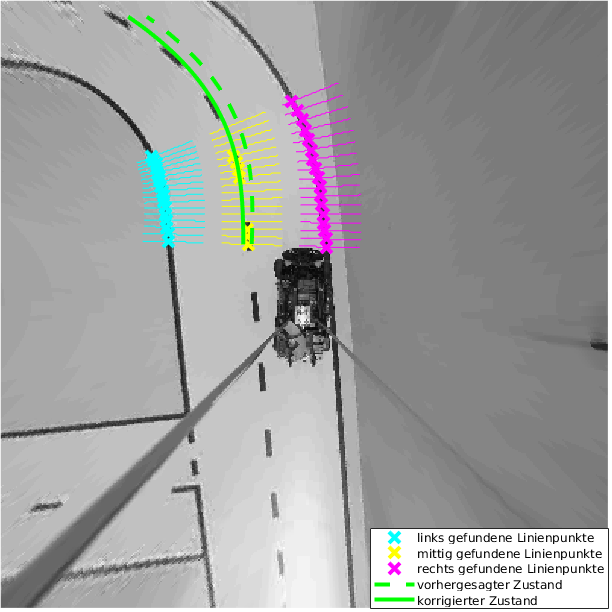
\includegraphics[width=0.75\textwidth]{kalman_iteration_komplett}
  \caption{Plot einer Iteration des Kalmanfilters}
  \label{fig:kalman:iteration_komplett}
\end{figure}

\subsection{konkrete Implementierung des Kalman-Filters}
Ist der \glsdesc{lat:statevector} \gls{lat:statevector} einmal wie in ~\ref{sssec:fahrspurerkennung:kalman:fahrspurmodell:initialisierung} beschrieben initialisiert, können die Gleichungen des Kalmanfilters bei Eintreffen eines neuen Bildes wie folgt berechnet werden:
\begin{enumerate}
\item Bildung der \glsdesc{lat:systemmatrix} \gls{lat:systemmatrix} mittels der seit dem letzten Bild gefahrenen Distanz \begin{math} \Delta \gls{lat:xcoord} \end{math}
\item Prädiktion des \glsdesc{lat:statevector} \gls{lat:statevector}, d.h. der Lage der Fahrspurmarkierungen im aktuellen Bild anhand von \eqref{eq:kalmanprediction}
\item Messung der Lage der Fahrspur wie in \ref{ssec:fahrspurerkennung:kalman:messung}
erläutert
\item Bildung der \glsdesc{lat:outputmatrix} \gls{lat:outputmatrix} passend zur Messung wie in \ref{sssec:fahrspurerkennung:kalman-filter:zustandsraumbeschreibung:outputmatrix} beschrieben
\item Korrektur des \glsdesc{lat:statevector}s \gls{lat:statevector} unter Nutzung von \eqref{eq:kalmancorrection}
\end{enumerate}




